\subsection{PandaBoard (FM)}
\label{sec:panda}

\subsubsection{Overview}
\label{sec:panda-overview}
The modelcar hardware contains 4 PandaBoards intended for running the Engine Control Units (ECU) communicating with the SpeedDreams simulation, processing the simulation data and generating the servo commands.
While two PandaBoards are used by the simulation team to process the simulation data from SpeedDreams, another Panda\-Board is used by our team to process the hardware control commands described in \autoref{sec:mqtt-car-control}.


\subsubsection{Requirements}
\label{sec:panda-req}
The following tasks were derived from the initial project description for the component running on the PandaBoard:
\begin{itemize}
    \item \textbf{TP1}: Install Genode with Fiasco.OC
    \item \textbf{TP2}: Develop MQTT client
    \item \textbf{TP3}: Convert control commands into concrete servo values
    \item \textbf{TP4}: Generate control commands
\end{itemize}

\paragraph{\textbf{TP1}} Genode running on top of the Fiasco.OS microkernel is used as operating system for the PandaBoard.
While there were less issues with running Genode on the PandaBoard compared to the Raspberry PI, a linux userland implementation of the PandaBoard component is also available in the \texttt{old/linux} folder and was used during initial development and testing.

\paragraph{\textbf{TP2}} As described in \autoref{sec:rpi-req} the same MQTT client based on the mosquitto library was used for the Raspberry Pi and the PandaBoard.
The PandaBoard subscribes to the \texttt{car-control} topic, processes received messages and then publishes to the \texttt{car-servo} topic.

\paragraph{\textbf{TP3}} The main purpose of the PandaBoard component is the transformation of generic control commands (eg. steer left, break) to concrete servo values. The format of the input and output messages is described in \autoref{sec:api} while the transformation is described in \autoref{sec:panda-genode}

\paragraph{\textbf{TP4}} To test the application independently of the SpeedDreams simulation, control commands can also be supplied directly as described in \autoref{sec:panda-testing}


\subsubsection{Genode application}
\label{sec:panda-genode}
The Genode application on the PandaBoard consists of two separate tasks communicating over IPC. The \textit{Main} task handles initial setup and network communication while the \textit{Control} task is responsible for the transformation of control commands to concrete servo commands. The interaction between these components is visible in \autoref{fig:panda-genode}.

\begin{figure}[h]
    \centering
    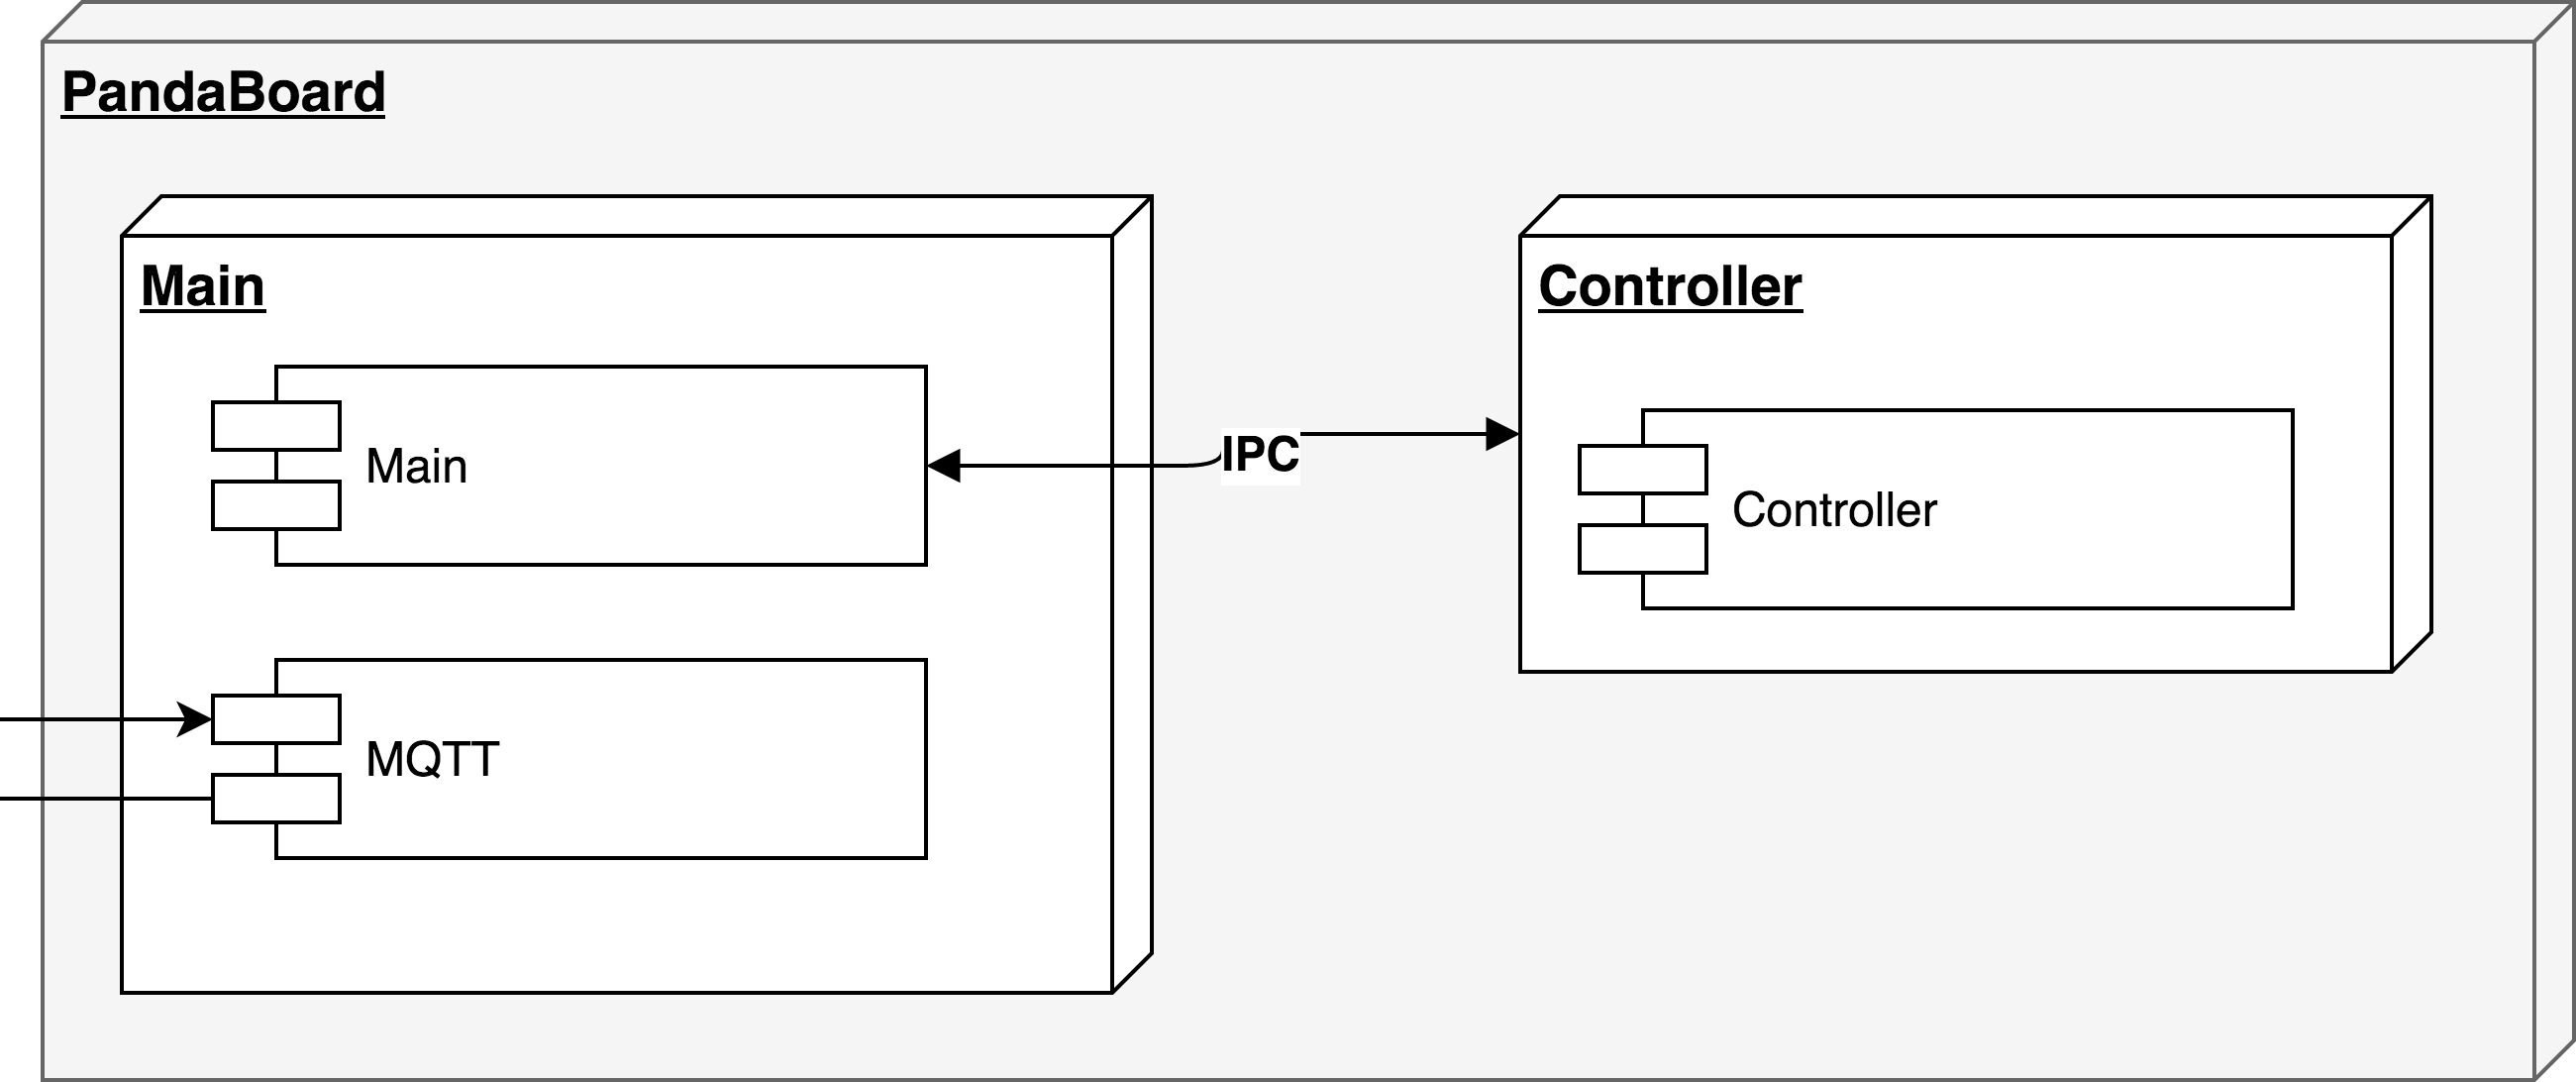
\includegraphics[width=0.7\linewidth]{images/comp_panda}
    \caption{Genode components of the PandaBoard}
    \label{fig:panda-genode}
\end{figure}

The runfile (\texttt{run/car\_panda.run}) contains the build and runtime dependencies as well as configuration settings for individual components.

After startup the \textit{Main} task reads the network configuration from the runfile and configures the network accordingly with either a static IP address or a IP address dynamically obtained over DHCP.

Afterwards it retrieves the IP of the MQTT server from the runfile and attempts to establish a connection.
The task then subscribes to the \textit{car-control} MQTT topic which causes all messages that are published on this topic to be forwarded to the application.

A callback that is executed on reception of every message then copies the data to a buffer where it is in turn processed by the main loop of the task.
After parsing the type of the message, the command is then sent to the responsible function of the \textit{controller task} over IPC.

As all IPC under Genode is synchronous, the \textit{Main} task resumes execution after the function call from the \textit{controller} task returns with the servo adjustment value obtained from the processed command.
The servo value is then published to the \texttt{car-servo} MQTT topic to which the \textit{Raspberry PI} is subscribed and handles all further processing.

% Advantages of genode task

\subsubsection{Command processing}
\label{sec:panda-convert}
The \textit{Control} component is responsible for transforming the messages received in an hardware independent format as described in \autoref{sec:mqtt-car-control} to concrete servo values suited for the servos built into the model car.

\autoref{lst:panda-tsteer} contains the algorithm for calculating the steering servos commands.
First the input value is checked to verify it is within the acceptable input range.
The value is then inverted to ensure correct mapping from the steering direction to the servo direction.
Afterwards the value is transformed by first adjusting the range to $0-1$ and then mapped to the servo input range by multiplying it with the input range of the servo (\textit{SERVO\_UPPER\_BOUND - SERVO\_LOWER\_BOUND}) and then adding the minimum servo value \textit{SERVO\_LOWER\_BOUND}.

As described in \autoref{sec:servo-hard} the minimum servo value is 4000 and the maximum servo value is 8000.
After testing the \textit{SERVO\_LOWER\_BOUND} was set to 4500 while the \textit{SERVO\_UPPER\_BOUND} was set to 7500 to prevent an actuation of the servos beyond the actuation limits of the attached hardware. \\

\begin{minipage}{\linewidth}
\begin{lstlisting}[style=mylistings, language=c, label=lst:panda-tsteer, caption=Algorithm for  calculating the steering servo commands]
int transform_steer(double value) {
	if (value < -1 || value > 1) {
		PERR("Invalid steering angle - range is -1 to 1");
		return -1;
	}

	// Invert value as SpeedDreams thinks -1 is right
	value = -value;

	value = (value + 1)/2;
	return (SERVO_UPPER_BOUND - SERVO_LOWER_BOUND) * value + SERVO_LOWER_BOUND;
}
\end{lstlisting}
\end{minipage} \\

%\begin{minipage}{\linewidth}
%\begin{lstlisting}[style=mylistings, language=c, label=lst:panda-tbreak, caption=Algorithm for calculating the break servo commands]
%int transform_brake(double value) {
%	if (value < 0 || value > 1) {
%		PERR("Invalid target brake position - range is 0 to 1");
%		return -1;
%	}
%
%	return (SERVO_UPPER_BOUND - SERVO_LOWER_BOUND) * value + SERVO_LOWER_BOUND;
%}
%\end{lstlisting}
%\end{minipage} \\


While the current controller only transforms the servo commands and forwards them, the design would also allow more high-level commands from the simulation to be processed where a single control \texttt{car-control} command generates a series of \texttt{car-servo} commands.
One example for this would be ABS style actuation of the servos and relying on sensor data to control the breaking strength.
As no suitable sensor measurements were available during this project, this part has not been implemented.

\subsubsection{Testing}
\label{sec:panda-testing}
To verify the data processing and the actuation of the hardware servos based on control commands sent to the \texttt{car-control} MQTT topic a test script was developed.
This way the hardware side of the HIL setup described in \autoref{sec:intro} can be tested independently of the software side developed by another project team.

The publish–subscribe pattern used by the MQTT server allows multiple clients to simultaneously connect to the server and subscribe to updates on a certain topic or publish messages to a topic.
In this style of communication there are no direct communication links and the components are loosely coupled, simplifying the testing of the interfaces between components.

By using the MQTT commandline tools available under Linux in the \texttt{mosquitto-clients} package message can easily be injected into the \texttt{car-control} topic without changing the configuration of any components.
\autoref{lst:panda-msgpub} shows a small test script that continuously sends steering control messages that cause the steering servos to alternate between actuation to the left and to the right. \\ % when processed by Panda, Rpi and servo components.

\begin{minipage}{\linewidth}
\begin{lstlisting}[style=mylistings, language=c, label=lst:panda-msgpub, caption=Injecting steering commands over MQTT]
#!/usr/bin/env bash
MQTT_IP=$1

while true; do
	mosquitto_pub -h $MQTT_IP -t 'car-control' -m '0,1.0'
	sleep 1
	mosquitto_pub -h $MQTT_IP -t 'car-control' -m '0,-1.0'
	sleep 1
done
\end{lstlisting}
\end{minipage} \\

In a similar manner the \texttt{mosquitto\_sub} commandline tool can be used to subscribe to MQTT topics. This provides easy access to the communication between components for debugging and testing purposes.
\autoref{lst:panda-msgsub} shows the command used to monitor the message published by the panda component. In both listings \texttt{\$MQTT\_IP} is a variable containing the IP address of the MQTT server. \\

\begin{minipage}{\linewidth}
\begin{lstlisting}[style=mylistings, language=c, label=lst:panda-msgsub, caption=Subscribing to MQTT topics]
mosquitto_sub -h $MQTT_IP -t 'car-servo'
\end{lstlisting}
\end{minipage} \\
